%-------------------------------------------------------------------------------
% BOARD ENCODING
%-------------------------------------------------------------------------------
\subsection{Board encoding}
\begin{frame}{``Cogito" system overview}{Board encoding}

Board was encoded in first order logic format.

Each encountered state of the board is an object, while certain configurations 
deemed are attributes. A configuration is invariant with regards to translations 
and rotations.

\end{frame}

\begin{frame}{``Cogito" system overview}{Board encoding}
	\begin{minipage}{0.45\textwidth}
		\only<1|handout:0>{
			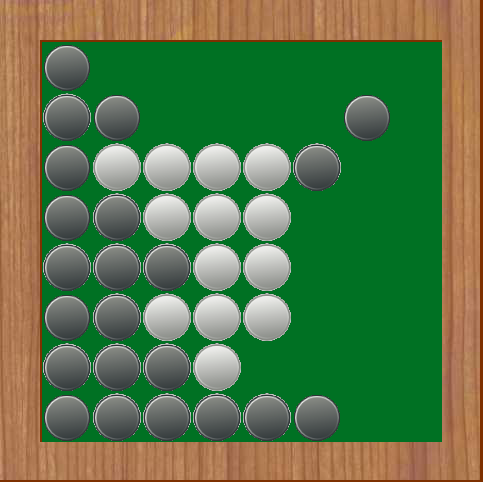
\includegraphics[width=0.8\textwidth]{img/cogito/raisonneur_choix_0}	
		}
		\only<2|handout:0>{
			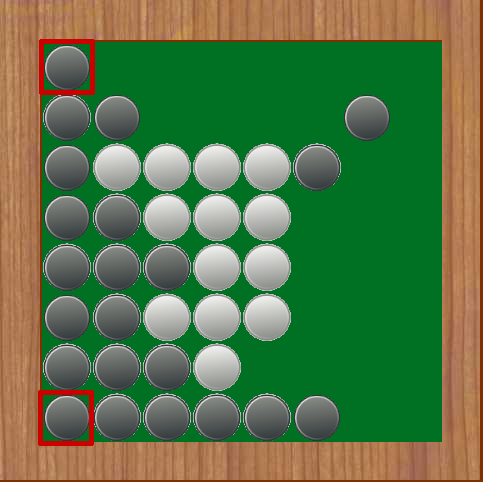
\includegraphics[width=0.8\textwidth]{img/cogito/raisonneur_choix_1}	
		}
		\only<3|handout:1>{
			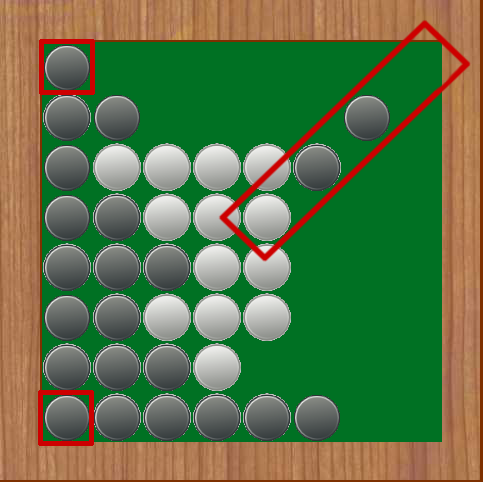
\includegraphics[width=0.8\textwidth]{img/cogito/raisonneur_choix_2}	
		}
	\end{minipage}
	\begin{minipage}{0.50\textwidth}
		\begin{itemize}
			\uncover<2->{
				\item $isCorner(x) \wedge isMine(x)$
			}
			\uncover<3->{
				\item $isMine(w) \wedge isOpp(x) \wedge isOpp(y) \wedge aligned(w,x,y) \wedge isEmpty(z) \wedge aligned (x,y,z)$
			}
		\end{itemize}
	\end{minipage}
\end{frame}

%-------------------------------------------------------------------------------
% MEMORY STRUCTURE
%-------------------------------------------------------------------------------
\subsection{Memory structure}
\begin{frame}{``Cogito" system overview}{Memory structure}
     
  \only<1|handout:1>{
    \begin{block}{Vision matricielle}
      \begin{center}
        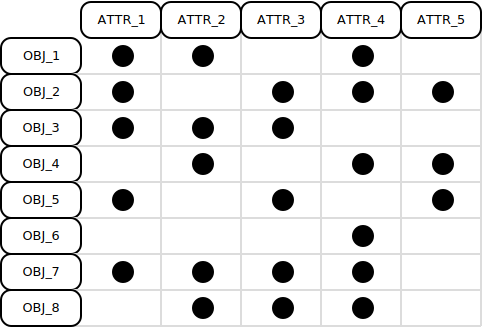
\includegraphics[width=0.6\textwidth]{img/cogito/context_matrix}
      \end{center}
    \end{block}
  }
  \only<2|handout:2>{
    \begin{block}{Vision en graphe}
      \begin{center}
        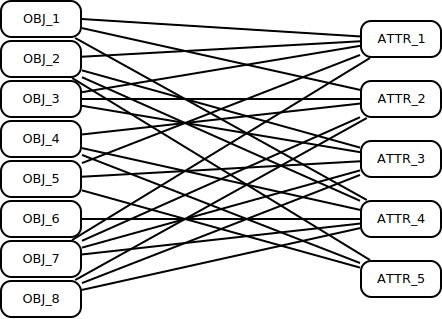
\includegraphics[width=0.6\textwidth]{img/cogito/context_graph}
      \end{center}
    \end{block}
  }
\end{frame}




%-------------------------------------------------------------------------------
% EVALUATING CONFIGURATIONS
%-------------------------------------------------------------------------------
\subsection{Evaluating configurations}
\begin{frame}{``Cogito" system overview}{Evaluating configurations}

When the game ends the final configuration is given a value based on whether the 
agent has won or last. This value and is propagated backwards through previous
board states with linear attenuation. The value of a state board the value 
of its configurations.

\end{frame}

%-------------------------------------------------------------------------------
% GENERATING NEW CONFIGURATIONS
%-------------------------------------------------------------------------------
\subsection{Generating new configurations}
\begin{frame}{``Cogito" system overview}{Generating new configurations}

New relevant configurations are deduced by attempting to locally extend an 
existing configuration shared by two or more winning or losing board states.

\end{frame}

%-------------------------------------------------------------------------------
% PUTTING IT ALL TOGETHER
%-------------------------------------------------------------------------------
\subsection{Putting it all together}
\begin{frame}{``Cogito" system overview}{Putting it all together}

The system receives a set of possible moves to choose from. By evaluating each 
resulting board state based on prior experience it is able to choose the one 
which seems most beneficial.

Nota Bene: there is no look-ahead, but as we are essentially engineering a 
dynamic heuristic the system could be easily combined with a limited-depth 
Minimax implementation.

\end{frame}